\documentclass{standalone}
\usepackage{pgfplots}
\usepackage{sansmath}
\pgfplotsset{compat=1.16}
\definecolor{bg}{HTML}{D8D8D8}
\definecolor{Display}{HTML}{1F77B4}
\definecolor{LowerExp}{HTML}{FF7F0E}
\definecolor{dtoa}{HTML}{2CA02C}
\definecolor{ryu}{HTML}{D62728}
\definecolor{teju}{HTML}{9467BD}
\definecolor{zmij}{HTML}{9C564B}
\tikzset{
  on layer/.code={
    \pgfonlayer{#1}\begingroup
    \aftergroup\endpgfonlayer
    \aftergroup\endgroup
  },
}
\pgfplotsset{
  every axis/.append style={
    x=12pt,
    height=3.5in,
    xmin=0.5,
    ymin=0,
    ymax=149,
    xtick pos=bottom,
    xtick distance=5,
    xticklabel shift=-1pt,
    tick label style={font=\sansmath\sffamily},
    every axis label={font=\sansmath\sffamily},
    label style={font=\sansmath\sffamily},
    ymajorgrids=true,
    major grid style={line width=0.8pt,draw=gray!55},
    axis background/.style={fill=bg},
  },
  every axis plot/.append style={
    line width=0.8pt,
    mark=*,
    forget plot,
  },
  area legend/.style={
    legend image code/.code={
      \draw[#1] (0cm,-0.1cm) rectangle (0.3cm,0.1cm);
    },
  },
  highlight/.style={
    preaction={
      on layer=pre main,
      line width=6pt,
      opacity=0.5,
      line cap=round,
      line join=round,
      yellow,
    },
  },
}
\begin{document}
\pagecolor{white}
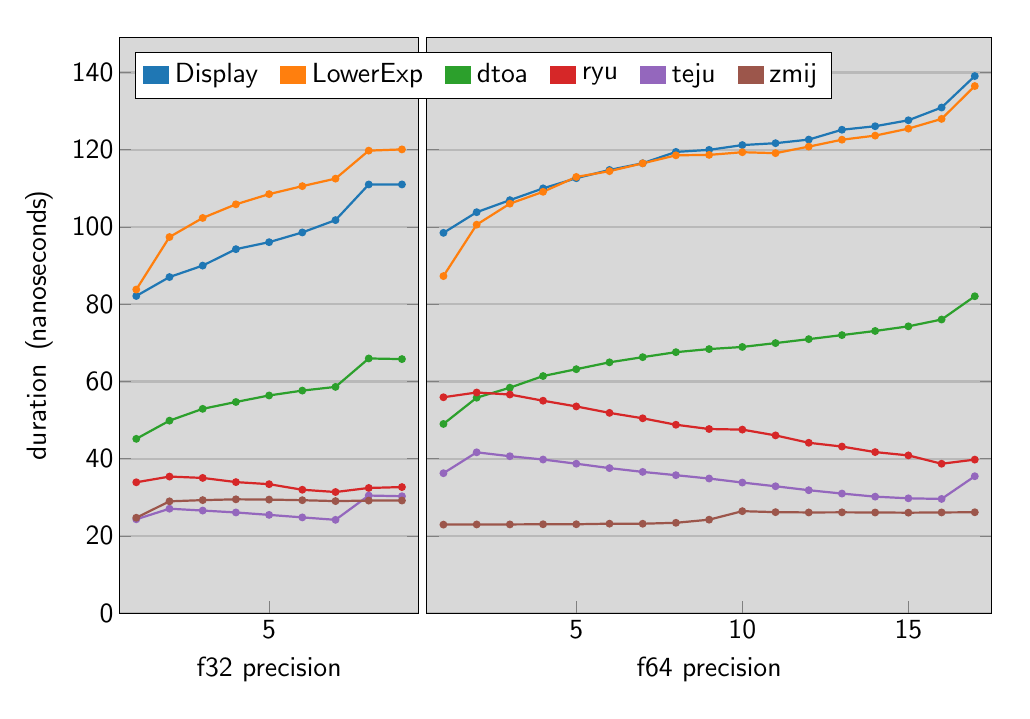
\begin{tikzpicture}[
  every mark/.append style={mark size=1pt},
]
\begin{axis}[
  name=f32,
  xmax=9.5,
  xlabel={f32 precision},
  ylabel={duration\enskip(\kern-1pt nanoseconds\kern-1pt)},
  yticklabel shift=-1.25pt,
  set layers,
  legend style={
    anchor=north west,
    at={(0.05,0.975)},
    font=\sansmath\sffamily,
    /tikz/every even column/.append style={column sep=6pt},
  },
  legend cell align=left,
  legend columns=-1,
]
  \addlegendentry{Display}
  \addlegendimage{color=Display, fill, area legend}
  \addplot[color=Display] coordinates {
    (1, 82.12)
    (2, 87.02)
    (3, 89.98)
    (4, 94.24)
    (5, 96.05)
    (6, 98.57)
    (7, 101.76)
    (8, 110.99)
    (9, 111.00)
  };
  \addlegendentry{LowerExp}
  \addlegendimage{color=LowerExp, fill, area legend}
  \addplot[color=LowerExp] coordinates {
    (1, 83.79)
    (2, 97.38)
    (3, 102.32)
    (4, 105.85)
    (5, 108.49)
    (6, 110.56)
    (7, 112.50)
    (8, 119.75)
    (9, 120.07)
  };
  \addlegendentry{dtoa}
  \addlegendimage{color=dtoa, fill, area legend}
  \addplot[color=dtoa] coordinates {
    (1, 45.13)
    (2, 49.84)
    (3, 52.90)
    (4, 54.67)
    (5, 56.36)
    (6, 57.62)
    (7, 58.58)
    (8, 65.94)
    (9, 65.78)
  };
  \addlegendentry{ryu}
  \addlegendimage{color=ryu, fill, area legend}
  \addplot[color=ryu] coordinates {
    (1, 33.88)
    (2, 35.36)
    (3, 35.01)
    (4, 33.93)
    (5, 33.39)
    (6, 31.95)
    (7, 31.36)
    (8, 32.41)
    (9, 32.64)
  };
  \addlegendentry{teju}
  \addlegendimage{color=teju, fill, area legend}
  \addplot[color=teju] coordinates {
    (1, 24.30)
    (2, 27.04)
    (3, 26.56)
    (4, 26.07)
    (5, 25.44)
    (6, 24.79)
    (7, 24.16)
    (8, 30.45)
    (9, 30.27)
  };
  \addlegendentry{zmij}
  \addlegendimage{color=zmij, fill, area legend}
  \addplot[color=zmij] coordinates {
    (1, 24.70)
    (2, 28.95)
    (3, 29.26)
    (4, 29.47)
    (5, 29.40)
    (6, 29.24)
    (7, 29.01)
    (8, 29.14)
    (9, 29.16)
  };
\end{axis}
\begin{axis}[
  name=f64,
  at=(f32.east),
  anchor=west,
  xshift=3pt,
  xmax=17.5,
  xlabel={f64 precision},
  yticklabel=\empty,
]
  \addplot[color=Display] coordinates {
    (1, 98.46)
    (2, 103.81)
    (3, 106.93)
    (4, 109.98)
    (5, 112.61)
    (6, 114.75)
    (7, 116.49)
    (8, 119.42)
    (9, 119.95)
    (10, 121.19)
    (11, 121.68)
    (12, 122.61)
    (13, 125.16)
    (14, 126.07)
    (15, 127.61)
    (16, 130.91)
    (17, 139.06)
  };
  \addplot[color=LowerExp] coordinates {
    (1, 87.27)
    (2, 100.58)
    (3, 106.02)
    (4, 109.09)
    (5, 112.94)
    (6, 114.44)
    (7, 116.46)
    (8, 118.54)
    (9, 118.65)
    (10, 119.34)
    (11, 119.10)
    (12, 120.79)
    (13, 122.58)
    (14, 123.64)
    (15, 125.45)
    (16, 127.97)
    (17, 136.47)
  };
  \addplot[color=dtoa] coordinates {
    (1, 48.98)
    (2, 55.78)
    (3, 58.37)
    (4, 61.39)
    (5, 63.16)
    (6, 64.94)
    (7, 66.28)
    (8, 67.57)
    (9, 68.37)
    (10, 68.92)
    (11, 69.92)
    (12, 70.94)
    (13, 71.99)
    (14, 73.06)
    (15, 74.26)
    (16, 76.02)
    (17, 82.05)
  };
  \addplot[color=ryu] coordinates {
    (1, 55.90)
    (2, 57.13)
    (3, 56.60)
    (4, 55.00)
    (5, 53.52)
    (6, 51.85)
    (7, 50.45)
    (8, 48.78)
    (9, 47.67)
    (10, 47.52)
    (11, 46.02)
    (12, 44.11)
    (13, 43.13)
    (14, 41.70)
    (15, 40.84)
    (16, 38.68)
    (17, 39.75)
  };
  \addplot[color=teju] coordinates {
    (1, 36.23)
    (2, 41.64)
    (3, 40.63)
    (4, 39.77)
    (5, 38.69)
    (6, 37.55)
    (7, 36.57)
    (8, 35.72)
    (9, 34.85)
    (10, 33.81)
    (11, 32.85)
    (12, 31.83)
    (13, 30.96)
    (14, 30.16)
    (15, 29.73)
    (16, 29.57)
    (17, 35.45)
  };
  \addplot[color=zmij] coordinates {
    (1, 22.92)
    (2, 22.96)
    (3, 22.97)
    (4, 23.01)
    (5, 23.01)
    (6, 23.16)
    (7, 23.15)
    (8, 23.39)
    (9, 24.20)
    (10, 26.40)
    (11, 26.15)
    (12, 26.07)
    (13, 26.10)
    (14, 26.06)
    (15, 26.01)
    (16, 26.07)
    (17, 26.12)
  };
  \legend{};
\end{axis}
\pgfresetboundingbox\path
  (f32.south west) -- ++(-0.46in,-0.39in)
  rectangle (f64.north east) -- ++(0.05in,0.05in);
\end{tikzpicture}
\end{document}
